To introduce our model and its biological basis this section we will start by introducing some fundamental biological concepts, before specializing in the science of fruit fly gastrulation. \\
We we will go through a short, broad explanation of the amount of information that is kept on cell- and embryo-level. Afterwards you will be introduced to the fascinating biology that allows each cell to partake in the creation of a complex living animal. Finally we will use all these newly learned concepts to introduce the model that our work will revolve around. By the end, we hope for every term and parameter in the model to seem sensible and biologically justified. 


\section{\hspace{-0.2cm}Broken Symmetries \& Genetic Patterning}
% \section{Everything}
\label{sec:theory-polarity}
\subsection{Broken Symmetries}
The interplay between order and symmetry is fundamental to any structured system. When a system develops complexity, it necessitates the breaking of an invariant, which arises from the disruption of symmetry.\cite{anderson1972more}
Symmetry breaking occurs at all levels of biological development, where small-scale ordering influence and shape the global symmetries of the organism. \\

Every organisms on this earth originate in the same way: A single, fertilized cell suspended in a liquid. Through mitosis this single unit copies itself,  creating an isotropic sphere. Suddenly, this ball will begin moving in a coordinated way to begin developing the shape of the organism to come. As animals are not spherically symmetric[citation needed], a number of symmetries need to be broken. \\

In Drosophila Melongaster, after the first rounds of mitosis, the cells begin sensing a chemical gradient in the yolk towards the shell which allows them to migrate and line the inside of the egg. This allows each of their surfaces to form distinct "outside" and "inside" domains. 
Preferential adhesion comes into play here, where cells can act selectively adhere to specific parts of their neighbors. 
Through preferential adhesion based on their relative surface orientation, the cells can maintain their positions and the overall structure of the shell, even in the absence of external support.
Thus our first symmetry break occurs, as this gives rise to the well defined embryo-scale inside-outside polarity. In biology this is known as \textbf{Apical-Basal polarity} which is observed in almost every multicellular system on the planet.\\

The second symmetry break is for breaking the up/down-symmetry. This happens differently for different animals, but the most well known example is found in the frog Xenopus, where the rotation of the egg, relative to the point of sperm entry, establishes this axis. In ways like this, the belly and back (Dorsal-Ventral axis) can be defined from fertilization.\\

Finally, we need some way of getting every cell to know an in-plane "forward" and "backward" direction. This polarity is called \textbf{Planar-Cell Polarity} and is almost as ubiquitous as the Apical-Basal polarity. In Drosophila, \textit{PCP} is defined through morphogens giving a clear (nematic) direction of high gradient. Morphogens, as predicted by Turing, are signaling molecules that help establish these asymmetries. These morphogens have distinct and stable patterning of low and high concentrations. When sensing these, cells can, using the previously broken symmetries, contribute to the creation of new morphogens. This coordination allows the cells to locally contribute to organizing global polarities and patterns.\\

The next step is to understand how these morphogen patterns emerge and how they lead to coordinated development across the embryo:



\subsection{Genetic Patterning}
\label{sec:gen_patterns}
For a multicellular organism to go from a homogeneous cell sheet to forming complex body plans, quite a bit of self-organizing is needed. The complicated interplay between cells necessitates both large-scale and cell-scale control. For human and fruit fly alike, this is done via genetic patterning.\cite{veraksa2000developmental}

As predicted by Turing, patterning is a result of "smartly"\footnote{Nature abhors a vacuous anthropomorphization} designed interactions where different chemicals assist or inhibit the production or expression of each other. These concentration gradients are both precise and robust enough to be picked up by the individual cells which allows for independent differentiation on a cell-by-cell basis.\\

% Now, to shake it up, \textit{Twist} \& \textit{Snail}, which might remind you of the beetles,\footnote{The species \textit{Tribozium} for example\cite{sommer1994expression}} are vital for the early development of a surviving fruit fly.

To get a feel for the amazingly complicated and remarkably precise patterning of these chemicals, four of them can be seen in Figure \ref{fig:MorphogenMap} below:


\noindent

\begin{figure}[H]
    \centering
    \makebox[\linewidth]{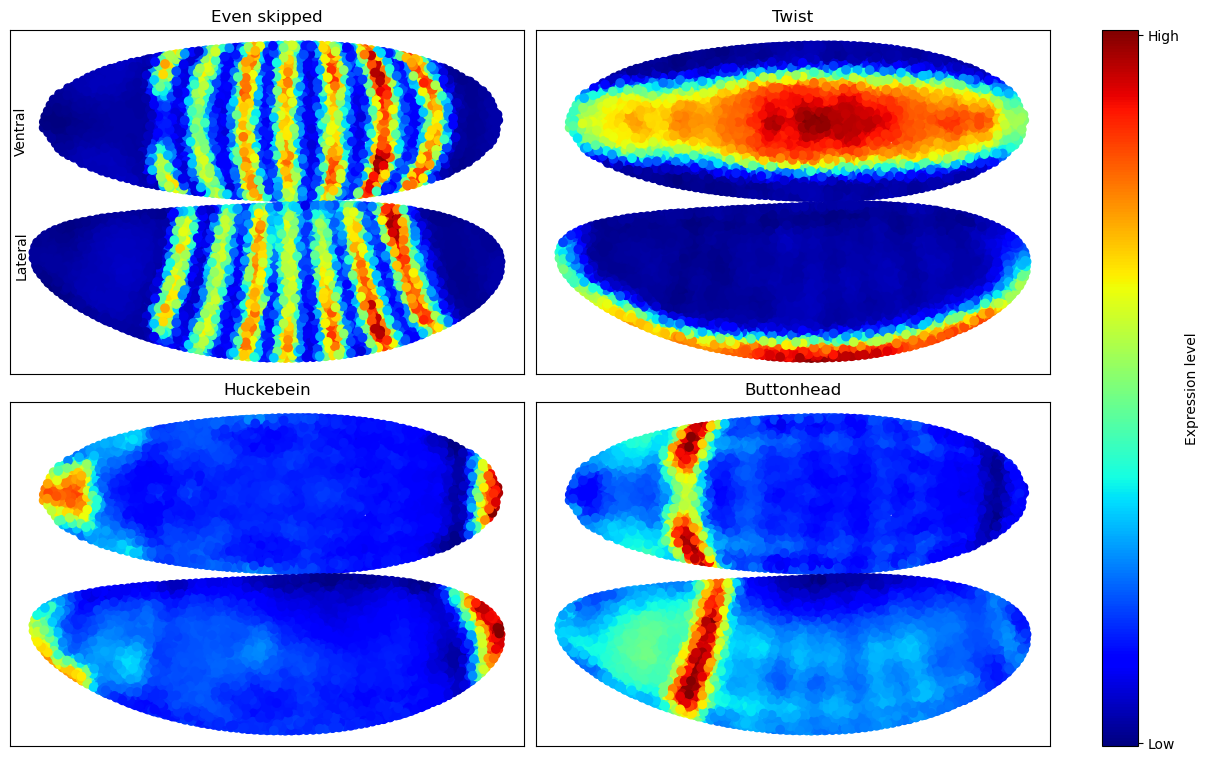
\includegraphics[width=1.\linewidth]{chapters/Theory/figures/patterning.png}}
    \caption{The spacial distribution of a small subset of morphogens. A clear attest to the remarkable and stable pattern formation Turing predicted chemicals gradients capable of producing.}
    \label{fig:MorphogenMap}
\end{figure}





For the complexity of macro scale morphology changes we observe, having off-equilibrium protein concentrations are not enough.  Luckily, the interaction between morphogens and mechanical deformations go both ways. This means, that when cells move according to some defined polarity, they can move the signal with them and break other cells' symmetries along the way. 

Each cell has local distribution YYY \todo{lay down base for polarizations}

It has been shown [citation needed] that a mechanical stimulus can trigger a chemical signal, thereby reinducing patterning in a feedback loop. This is called \textbf{mechanotransduction} and is believed to be vital in (for example) stable PCP-orientation. A relevant example of mechanotransduction is how cells can sense movement from a particular direction and respond by aligning themselves accordingly. This alignment can trigger a cascading effect, ultimately contributing to the overall shaping of the tissue.\\


Let us take a small step back and think how extraordinary this all is. Every individual action is transcribed from the same string of DNA, where nothing happens except building one of 20-ish amino acids to form proteins. These proteins can then either help or delay the transcription of the same DNA string. It is the order in which these simple proteins are created that, together with the simple physical self-interaction, allows for the exponentially more complex cell to emerge.


And now, the same thing happens on the next level: Individual cells will each be making simple mechanical alterations to their shape. The interplay between these can somehow arrive at a cohesive bigger picture. To understand this behaviour, we will need to look at the individual mechanisms:

\section{How Cells Move}
\label{sec:howmove}
Most of the global, large-scale motion seen during development of any multicellular organisms stem from a handful of seemingly simple, albeit still not well understood, active single-cell actions.\cite{walck2014cell}\\

In most cases, cell migration consist of chemotaxis. That is, individual cells moving in the direction of a chemical gradient.\\
What we will be looking at is fundamentally different. In embryogenesis, where cells are closely bound together in epithelial sheets, the cells are able to exert forces on \textit{each other}. As can be seen on Figure \ref{fig:mysosinMeshwork}, the cells stay interconnected using membrane tethers connecting local neighborhoods. This means every cell can change its shape relative to its bordering cells allowing for combined motion more efficient than any single cell could achieve on their own.[cite video] 
% When thinkin of cell motility, chemotaxis 

% The motion we will be looking at, are of a type that is fundamentally different from Chemotaxis, with cells reacting to a local chemical concentration but not moving along a gradient [citation needed].

% The cells internal structure is called the cytoskeleton with internal \textit{motor proteins} responsible for keeping and changing the cells shape.
\begin{figure}[H]
    \centering
    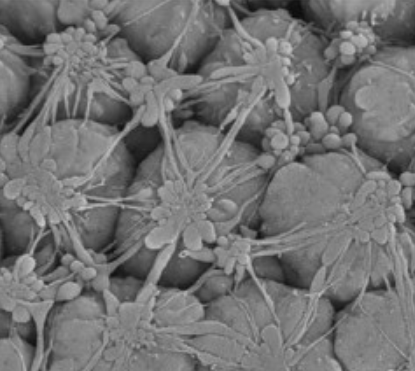
\includegraphics[width=0.6\linewidth]{chapters/Theory/figures/EM_constricting_proteins.png}
    \caption{Electron microscopy of\textit{ Myosin II}-protein meshwork on the belly-side of the fruit fly embryo. (Source: \citeAY{martin2010integration})}
    \label{fig:mysosinMeshwork}
\end{figure}


Studying these 'local motions with global consequences' is the main point of focus for us. Unfortunately experimenting with living cells is inherently hard, which means that in Drosophila gastrulation, these 'driving effects' are surprisingly under-understood with no paper claiming to have an exhaustive list. Here is some of the fundamental single-cell active forces that are undeniably happening:

\textbf{Convergent Extension} and \textbf{Apical Constriction}

\subsection{Convergent Extension}
\label{sec:ConvergentExtension}
For elongating of sheets in a single direction, \textit{Convergent Extension} seems to be one of the most common proprietors of movement. It is made up of asymmetric cellular intercalations. In layman's terms: Cells squeezing in between each other, but mainly in one direction. 
In Figure  \ref{fig:cellIntercolation} a schematic of how cell intercalation can lead to extension can be seen.
\begin{figure}[H]
    \centering
    \begin{subfigure}{0.45\linewidth}
        \centering
    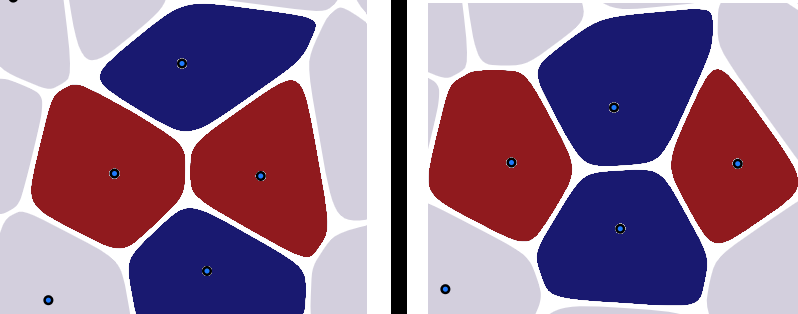
\includegraphics[width=\linewidth]{chapters/Theory/figures/ConvergentExtensionDiagram.png}
    \caption{}
    \label{fig:cellIntercolation}
    \end{subfigure}
        \begin{subfigure}{0.45\linewidth}
        \centering
    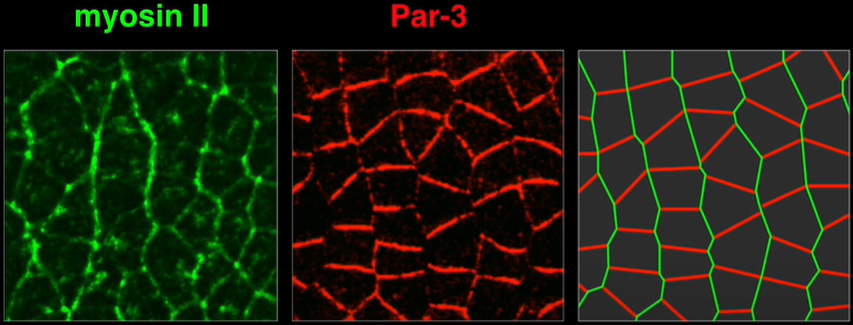
\includegraphics[width=\linewidth]{chapters/Theory/figures/bipolar-PCP.png}
        \caption{}
    \label{fig:dyedDifferentialWall}
    \end{subfigure}
    \caption{\textbf{(a)}: A diagram showing how guided intercolation of blue cells can results in horizontal elongation of the cluster \\\textbf{(b)}: Dyed Germ Band tissue showing clear difference in horizontal and vertical protein expressions (Source: \citeAY{zallen2004patterned})}
    
    \label{fig:ConvergentExtensionDiagram}
\end{figure}

The Planar-Cell polarity, as described in the previous section, can gives rise to a stark difference of protein concentrations between horizontal and vertical cell walls. This can be seen in Figure \ref{fig:dyedDifferentialWall}.
Through anisotropically tightening of cell borders, with deformations only happening in the individual cell, the full sheet can change shape. No cell even needs to know its position in space or barely change its shape. 

This contraction on a specific side of a cell, leads us to the next fundamental active force.



\subsection{ Apical Constriction }
\label{sec:ApicalConstriction}
When the cell sheet wants out-of-plane bending, they turn to Apical Constriction. Apical constriction functions exactly as you would think; Protein rings constrict the apical (outer) side of the cell, creating a smaller surface area. This leads to bending and, when enough constriction is applied, invagination. (see Figure \ref{fig:apical-constriction}). Cells have shown the ability to constrict both isotropically and anisotropically (relative to the Planar-cell Polarity) granting cell-sheets the ability to form both valleys and cavities.

\begin{figure}[H]
    \centering
    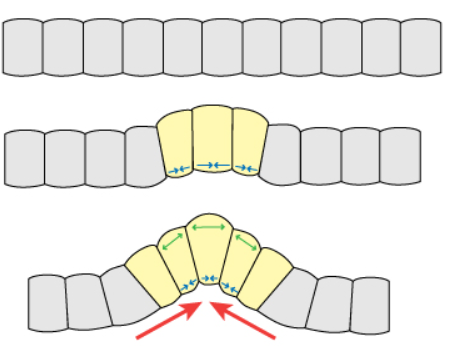
\includegraphics[width=0.3\linewidth]{chapters/Theory/figures/apical_constriction_schematic.png}
    \caption{Schematic for how apical constriction works (Source:\todo{})}
    \label{fig:apical-constriction}
\end{figure}

% \subsection{Cell Shape Change}
% At the onset of gastrulation, the cells are tightly packed, giving them a pronounced elongated shape. The cells can use their cytoskeleton to actively reshape their in-plane area quite drastically. [citation needed]

% \subsection{Proliferation}
% If cells are dividing in-plane, they can apply a pressure. In the stages of we are looking at, cell-division is shown to not be a driving force except in the head-region. [citation needed] As this has not been simulated in the final iteration.\\

Now, the fact that nature is thrifty with its creations, means, the few actions described above is used in the creation of almost every type of organ in almost every type of organism. The hope is, that understanding these fundamentals in one system might allow for lessons to be learned in another. In this thesis we will focus on the motility required for Drosophila gastrulation to [arise]. As explained in the introduction, The fruit fly is a model organism, and the fact that it has been observed by biologists for years makes it a great onset for probing the intricacies of biomechanics.\\



To summarize what we have learned:
Through \textit{genetic patterning} and other \textit{broken symmetries} both the embryo on the whole and each each cell has protein gradients, and, through the distribution of these, well-defined \textit{polarities}.
Through \textit{mechanotransduction}, \textit{local movements} can be tied to these polarities and vice versa, allowing for stable, global morphological changes to occur. Examples of these local driving forces are \textit{convergent extension} and \textit{apical constriction}. \todo{cut?}


Now, what is a fruit fly? 

% \section{Drosophila in Detail}
% Before we can get to the model it is necessary to introduce the star of the show. We will start out by YYY the features of the embryo before we move on to the motions it undergoes. 
% \subsection{The Drosophila Embryo in detail}
% \label{sec:drosophila-embryo-detail} 
% We will quickly outline the main morphological features of the gastrulation cycle of the embryo:
% \begin{outline}
%     \1 Posterior Midgut (PMG)
%     \1 Anterior Midgut (AMG)
%     \1 Ventral Furrow
%     \1 Dorsal Transverse Furrows
%     \1 Cephalic Furrow
%     \1 Germ Band
% \end{outline}

% \begin{figure}[H]
%     \centering
%     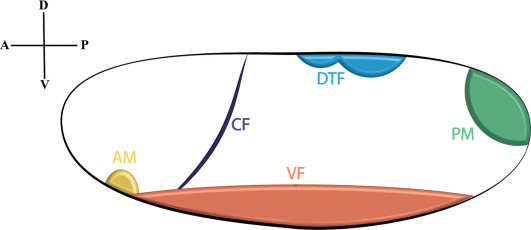
\includegraphics[width = 0.7\linewidth]{chapters/Theory/figures/morphogenic_events.jpg}
%     \caption{Summary of the morphogenetic events mapped onto the blastoderm stage embryo. Taken from \cite{gheisari2020gastrulation}. The colored parts are generally seen to be the morphogenetically active during the early part of the embryogenesis}
%     \label{fig:enter-label}
% \end{figure}

% IN OUR SIMULATION: 

% The Germ Band is defined as all cells expressing a sufficient YY of the two striped genes \textit{Eve} and \textit{Run} the at the onset of gastrulation. \cite{zallen2004patterned}


\newpage
\section{The Drosophila Gastrulation in detail}
In the literature, the development of the fruit fly from fertilised egg to hatched larvae is usually divided into 17 distinct events.\cite{bownes1975photographic} We will be looking at stages 5 through 7, lasting about 15 minutes. These are characterized by having the first mesoscopic morphogenetic movements and setting the stage for all morphology to come.

The egg has a radius of about 1/10th of a milimeter\footnote{Source: This wonderful website: \url{https://bionumbers.hms.harvard.edu/bionumber.aspx?id=111360}}
After 12 rounds of cell division with about the egg now consist of about 5000 cells. 
When looking at the embryo, the following parts will be the most active, important and relevant to our project:


% \begin{figure}[H]
%     \centering
%     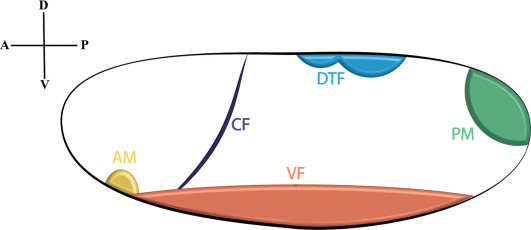
\includegraphics[width = 0.9\linewidth]{chapters/Theory/figures/morphogenic_events.jpg}
%     \caption{Taken from \citeAY{gheisari2020gastrulation}. \\
%     VF: Ventral Furrow\\
%     PMG: Posterior Midgut\\
%     CF: Cephalic Furrow\\
%     Germ-band: A band of germs}
%     \label{fig:enter-label}
% \end{figure}

Now, the gastrulation can begin.
The Drosophila gastrulation consist of a series of interconnected but independent cell movements.\\
We will now present an abridged overview, roughly ordered in time:





\newpage

\begin{figure}[H]
    \centering
    \vspace*{-1cm}\makebox[\textwidth]{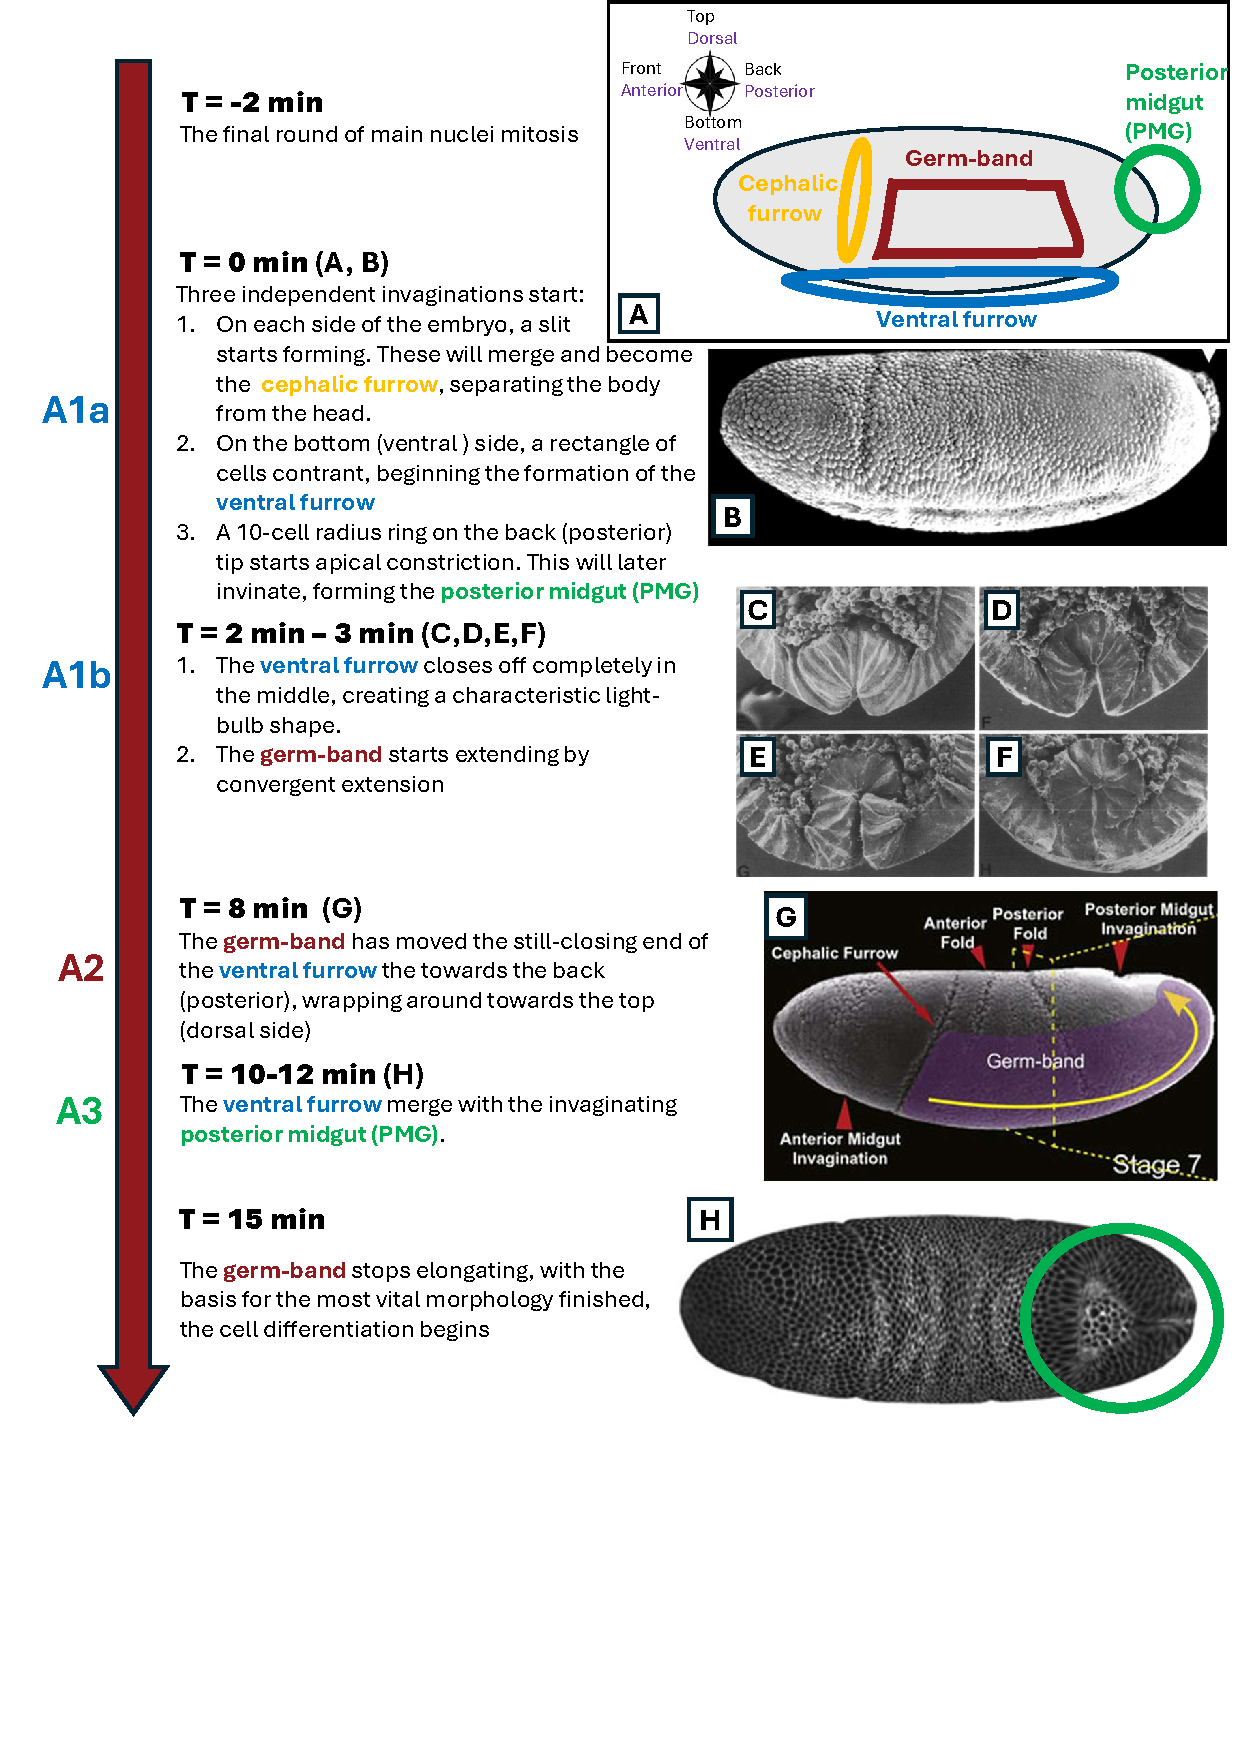
\includegraphics[width=0.8\paperwidth]{chapters/Theory/figures/Timeline_v2.pdf}}
    \caption{Caption}
    \label{fig:big-timeline}
\end{figure}
\newpage
\addtocounter{figure}{-1}
\begin{figure} [t!]
  \caption{
  \textit{(Previous page.) }\\ 
  A somewhat comprehensive explanations of the most important parts of the early Drosophila gastrulation. The three events (\vf{A1}, \gb{A2} and \pmg{A3}) have been highlighted by us. These has been chosen as being both fundamental for the final morphological outcome and relating to different domains of the embryo.\todo{Add reference?}\\
  \textbf{A:} A diagram of the drosophila embryo as it is usually depicted: The front side (what will become the head) facing left. The primary domains of interest are depicted. (Source: )\\
  \textbf{B:} An electron miscroscope image of the at around 30 sec. On the anterior (back) tip, a number of germ cells (called pole cells) can be seen. These were not part of our simulation even though it has been shown that that have both mechanical and chemical interactions during gastrulation. (Source: )\\
  \textbf{C-F:} Electron microsopy of the \vf{ventral furrow} closing off. (Source: )\\
  \textbf{G:} A diagram of the motion of the \gb{germ-band} as it extends. The locations of auxiliary folds are also highlighted. (Source: )\\
  \textbf{H:} A [type of microspcopy] showing the \pmg{posterior midgut} as it invaginates and combines with the ventral furrow.

  }

\end{figure}
% \vspace*{5cm} 

As we now have the basis for understanding how ...

\todo{Reexplain problems}
% \textit{This page is intentionally left blank so the previous page can be taken and kept as a cheat-sheet for later referencing. }
\newpage
\section{Previous attempts at simulation}
\note{I am aware this section is not up to par :)}\\
In silico models has already provided multiple working examples of all the aforementioned embryogenetic events with multiple different approaches since the 1970's.\\
When studying the biomechanics of morphogenesis there seems to be two primary strategies:\\

\textbf{Top-Down Approach:} This strategy focuses on a single morphogenetic event, modeling it in detail. For instance, ventral furrow formation can be simulated as an elastic sheet subjected to pulling forces \todo{find reference}. This approach can enhance our understanding of the physical forces or biological systems required for the event to occur but may limit generalization to other morphogenetic processes.\\

\textbf{Isolated Active Phenomenon:} In this approach, a single active phenomenon, such as convergent extension, is simulated "in a vacuum." This allows for a detailed comparison of the actions of individual cells against imaging of YYY. An example of this could be the YYY,.  This method can provide great insight into the underlying physics and chemistry at play. However, this method may fall short in shedding light on the any specific morphogenetic event or omit important context.\\

It is mainly either vertex-based or continuum approximation-based simulations that have dominated the field. These are all great for accurately describing the minute changes in the physics of tubologenesis, tissue-folding etc., but they comes with some drawbacks. These  models focus on the pressure and tensile forces, simulating the strains in the cell walls. Finite-element models that look at sub-parts of cells are often computationally heavy. This often requires it to be done in 2D \cite{krajnc2018fluidization}, inherently loosing some particularities of the problem. A more computationally efficient approach is the cell-center based models. When looking for off-lattice center-based model, not many show up. An example, but only using non-polar interactions is \citeAY{atwell2015mechano}. They modeled who modeled \todo{finish}.\\

This all boils down to: No one has been able to simulate the formation of the posterior midgut (\pmg{A3}), as this requires a successful model of (\vf{A1}) and (\gb{A2}), and a way to combine them, almost necessitating a simulation of the full embryo.


% Examples of 1) are early Apical Constriction 2d cross section \cite{odell1981mechanical}, 

% 

% State-of-the-art vertex based compared to other types \cite{fletcher2017mechanocellular}

% The problem is, that [Avogadro constant] is quite large. 

% This allows for a , but the interplay between different parts of the embryo, different [force-types] and YYY are ignored.  


% Removing the focus from the on the biomechanics of a single part, instead focusing on the YYY, Just like nature is reusing\\\\

% \textbf{All of this means,} 




This all leads us to the star of the show:

\section{The Model}

Our model takes its onset in the ideas posed in \citeAY{nissen2018theoretical} and later expanded in \citeAY{nielsen2020model}. Whenever we deviate from the existing literature, this will be stated clearly.\\

As we know global-scale changes in physical structure during gastrulation all arise from single cell actions with little discernible individual movement. The model is built around simulating the cells as point-based particles and elevate their individual [chemical?] gradients to vectors with explicitly stated orientations. No global YYY, no YYY stresses or strains, no YYYY. \\
It is based on the following intercellular potential $V_{ij}$ described by: 

\begin{equation}
    V_{ij}=e^{-r_{ij}}-A_{ij} e^{-r_{ij}/\beta}
    \label{eq:main-pot}
\end{equation}

Where $r_{ij}$ is the distance between two cells $A_{ij}$ is a attraction factor that will be explained later, and $\beta$ is a constant that sets the scale between these two. The first term is a short range repulsion preventing them from overlapping and the second is a long range attraction defining their interactions. The constant $\beta$ (usually set to 5, which is very constant) effectively defines the cell size for a given $A_{ij}$. 

Now, every individual cell \textit{i} tries to minimize the quantity 
\begin{equation}
    U_i = \sum_j V_{ij}
    \label{eq:totalPot}
\end{equation}
where the sum over $j$ is over all Line of sight/Voronoi neighbors. Voronoi neighbors are cells that share a boundary in a Voronoi diagram (see Figure \ref{fig:voronoi-explanation}). 

\begin{figure}
    \centering
    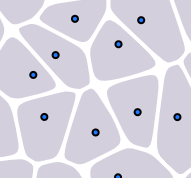
\includegraphics[width=0.25\linewidth]{chapters//Theory//figures/voronoi_explanation.png}
    \caption{A Voronoi diagram. Every point within a region is closer to its respective \textit{cell} than to any other \textit{cell} in the space.\todo{some other word for cell}. The regions are drawn with rounded corner for no other reason than  to make it look more like biology.}
    \label{fig:voronoi-explanation}
\end{figure}
The interaction across cellular neighbors should remind you of the nearest-neighbor protein connections in Figure \ref{fig:mysosinMeshwork}. 
\todo{Reexplain myosin or remove note}\\

To get a feeling for $S_{ij}$ (Equation \ref{eq:main-pot}), the potential can be seen in Figure \ref{fig:potential} for $A_{ij}=1$.
\begin{figure}[H]
    \centering
    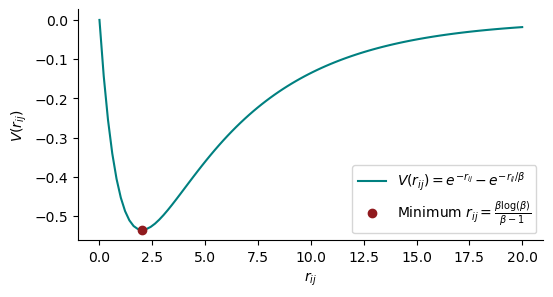
\includegraphics[width=1.\linewidth]{chapters/Theory/figures/potential.png}
    \caption{The potential well our point particles lie in, with the minimum (i.e. effective cell size) drawn in. Here we also see the role of $\beta$ as responsible for regulating the relaxation-distance}
    \label{fig:potential}
\end{figure}

The shape of the potential well should remind you of the Yukawa/Lennard-Jones potential, which also rely on strong short-range repulsion and weaker, longer-ranged attraction.\\

Running the simulation at this point, the cells would simply converge to a sphere. Much like the earliest stage of the Drosophila embryo.


% Lets us introduce these new $S$-terms one by one, keeping the biological foundation we built up in the earlier sections in mind:\\

% We would want a simple term that allows for non-polar attraction between cells. We start out by defining $S_0$: 
% \begin{equation*}
%     S_0 = 1
% \end{equation*}



Now, just like in nature, some symmetries needs to be broken to allow for interesting morphologies to emerge.\\
The principal idea is to elevate the Apical-Basal and Planar-Cell polarities (as described in previous sections) by seeing them as explicitly stated polarization vectors with rules for intra- and inter-cell interactions. 

Mechanotransduction refers to the process by which cells convert mechanical stimuli into biochemical signals.

The first symmetry that is broken is the inside-outside symmetry. Introducing the (normalized) $\hat{p}$ vector for each cell allows for emulation of the \textit{Apical-Basal} polarity.
As previously mentioned the interplay between cell-polarisation and physical orientation goes both ways (the mechanotransduction as described in section \ref{sec:theory-polarity}).
\todo{reexplain mechanotransduction adn hwo cells have polarities etc}
This motivates the following term which I will explain after introducing:

\begin{equation*}
    S_1=\left(\hat{p}_i \times \hat{r}_{i j}\right) \cdot\left(\hat{p}_j \times \hat{r}_{i j}\right)
\end{equation*}

$S_1$ ties the relative positions between a cell and its neighbors $\hat{r}_{i j}$ to their respective AB-polarities $\hat{p}$.
As can be seen, this is a dot-product of cross products. This configuration can be understood for $\left(a \times b\right) \cdot\left(c \times d\right)$ as "keep a and c, and b and d respectively parallel, while keeping a and b, and c and d internally perpendicular". \\ 

In the case of $S_1$, it encourages cells to lie in a plane, perpendicular to their AB-polarities. A diagram of the effects can be seen below (Figure \ref{fig:explain-S1}). Adding the $S_1$-term to our potential produces sheets of cells. 

% \begin{figure}[H]
%     \centering
%     \includegraphics[width=0.3\linewidth]{chapters/Theory/figures/explainS1.png}
%     \caption{A visual help for understanding the influence of the $S_1$-term (Equation \ref{eq:s1}). The orange arrow is the AB-polarity and the blue circles representations of the positions of the cells.}
%     \label{fig:explain-S1}
% \end{figure}

\begin{figure}[H]
    \centering
    \includegraphics[width=1\linewidth]{chapters//Theory//figures/explainS1.png}
    \caption{Enter Caption}
    \label{fig:explain-S1}
\end{figure}
\todo{An itroductpry sentence}
The second symmetry break is the planar polarization. We introduce the Planar-Cell-Polarities $\hat{q}$ (PCP from here on), and define the dynamics as follows:
\begin{equation*}
    S_2=\left(\hat{p}_i \times \hat{q}_{i}\right) \cdot\left(\hat{p}_j \times \hat{q}_{j}\right)
\end{equation*}
This term keeps the PCP and AB polarities perpendicular within each cell, but aligned across cells. This gives a stable and consistent, but changeable in-plane orientation vector for each cell. A diagram can be seen in Figure \ref{fig:explain-S2}.\\
\begin{figure}[H]
    \centering
    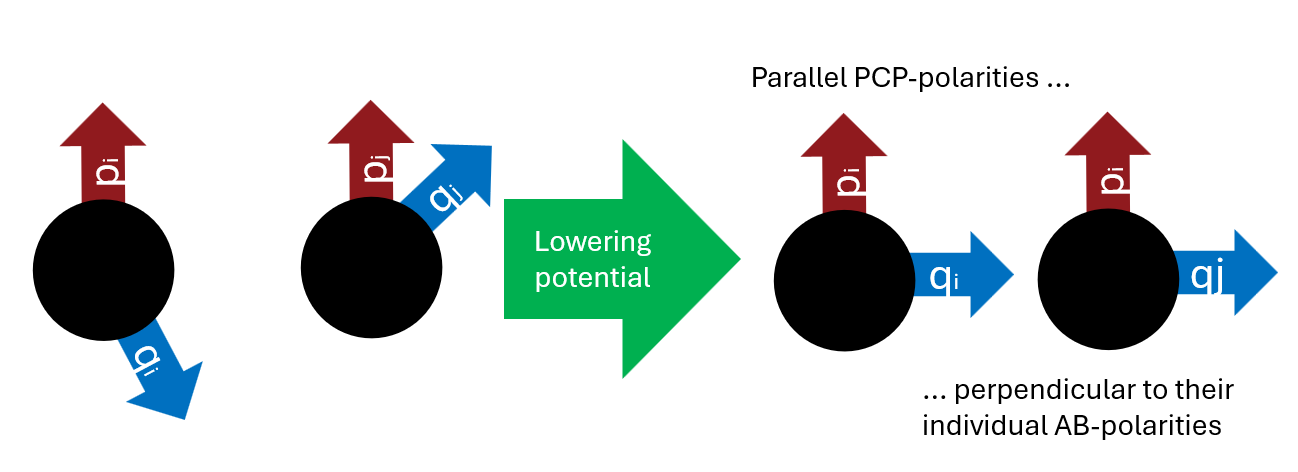
\includegraphics[width=1\linewidth]{chapters//Theory//figures/explainS2.png}
    \caption{Enter Caption}
    \label{fig:explain-S2}
\end{figure}
To take advantage of the this possible direction of motion, we will take inspiration from the Convergent Extension (Section \ref{sec:ConvergentExtension}) and introduce the final step of the dynamics, coupling the cells relative positions with their PCP-vectors. While we \todo{something about not being completely like bio. From Nissen: our assumption of anisotropic, planar polarized adhesion.}

\begin{equation*}
    S_3=\left(\hat{q}_i \times \hat{r}_{i j}\right) \cdot\left(\hat{q}_j \times \hat{r}_{i j}\right)
\end{equation*}

This term is lowest when the Planar-Cell-polarities are aligned but perpendicular to their relative direction-vector. In the realm where this term dominates, the cell sheets created by $S_1$ and $S_2$ are exchanged for lines of cells perpendicular to their PCP-vectors. 
\begin{figure}[H]
    \centering
    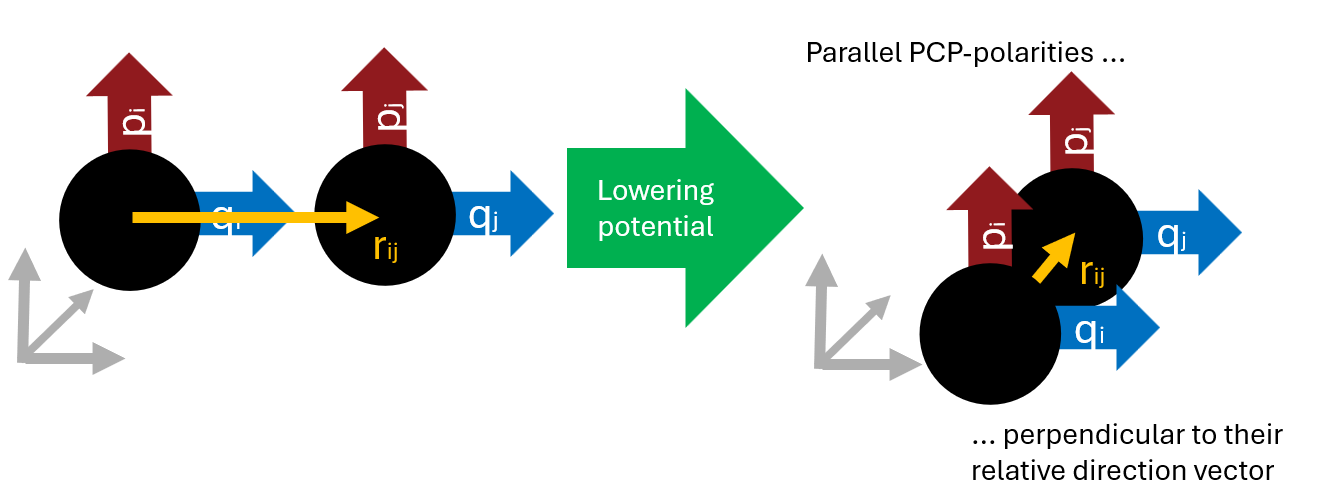
\includegraphics[width=1\linewidth]{chapters//Theory//figures/explainS3.png}
    \caption{Enter Caption}
    \label{fig:enter-label}
\end{figure}

While not biologically \todo{Write how this makes CE}

The full array is therefore:

\begin{subequations}
\begin{align}
S_0&=1\label{eq:s0}\\
S_1&=\left(\hat{p}_i \times \hat{r}_{i j}\right) \cdot\left(\hat{p}_j \times \hat{r}_{i j}\right)\label{eq:s1}\\
S_2&=\left(\hat{p}_i \times \hat{q}_{i}\right) \cdot\left(\hat{p}_j \times \hat{q}_{j}\right)\label{eq:s2}\\
S_3&=\left(\hat{q}_i \times \hat{r}_{i j}\right) \cdot\left(\hat{q}_j \times \hat{r}_{i j}\right)\label{eq:s3}
\end{align}
\end{subequations}


We can now finally introduce the more complicated $A_{ij}$-parameter as teased in Equation \ref{eq:main-pot}. We see it as a sum of the four previously described $S_i$-terms, each with an associated scaling factor $\lambda_i$ for  
\begin{equation}
    A_{ij}=\sum_{n=1}^{3}\lambda_n  S_n(r_{ij}, p_i, p_j, q_i, q_j)
\end{equation}


If the constraint $\sum_{n=1}^{3}\lambda_n=1$ is not fulfilled, the relaxed cell size is not constant. Importantly in implementation, the $\hat{p}_i$'s and $\hat{q}_i$'s are unit vectors and are therefore constrained to being normalized.\reph\\

To round off our array of actions the cells can take \reph, we introduce the second dynamical [smth],\footnote{Checkov's active single-cell biomechanics} described earlier: Apical constriction (Section \ref{sec:ApicalConstriction}). In our model, this is done via \textbf{Wedging}

As apical constriction is the single cells way of creating larger-scale furrows and wedges, we implement this by changing the $\hat{p}_i$'s to 'trick' each cell into believing their neighbors are differently oriented, thereby changing the relaxation angle:

\begin{equation}
    \tilde{{p}}_i = \frac{\hat{p}_i-\alpha \widehat{{r}}_{i j}}{|\hat{p}_i-\alpha \widehat{{r}}_{i j}|} 
\end{equation}

with $\alpha\in [0,0.5]$ 

\todo{add drawing}


A similar expression can be made for anisotropic wedging, taking  $\hat{q}_i$'s into account. All cells can now be defined by a cell type, which simply means they have a $\lambda$-array and a $\alpha$ associated with them. \todo{foreshadow?}\\


We will now, diverging from the original papers, and morph the basic model into something that is useful in for our specific case.\\

\textbf{Boundary conditions} where parameterized by hand from visual references and added as a simple term in the potential 

A slight \textbf{differential adhesion} was needed for the simulation to run smoothly. The interaction between the ventral furrow cells (cell type 2) and cells of other types where scaled by a factor of 5\% (multiplied by 0.95) so as to discourage unnecessary mixing. This is a phenomenon often seen in nature and is many ways already part of our model.\\

To emulate the lowering of apical surface area \textbf{better emulation of apical constriction} was introduced. Invaginating cells ($\alpha > 0$) got an increase in their $\lambda_1$'s (in Equation \ref{eq:s1}) making their relaxation distance shorter. This had the added benefit of echoing the tighter bonds in constricting cell clusters. [citation maybe needed]\\

\textbf{S1 -- S0}\\
When any of the invaginating tissue 'closed off' it forced cells on either side to have their AB-vectors pointing towards each other. A line of code was added, to combat this: When two apical sides interacted and  they were only allowed to interact as non-polar, i.e. their $S_1$-terms where changed into $S_0$.


\textbf{Nematic $S_2$ and $S_3$} write this

And finally, the most important contribution -- \textbf{Patterning}:\\
As we have about 5000 cells with four $\lambda$'s and a wedging constant $\alpha$ for each, this effectively gives 25000 parameters.

To combat this, we again look to nature and remember the patterning Section \ref{sec:gen_patterns}. Somehow all the information a cell needs will be in these boundary conditions.\\
Luckily for us, straight from Wikipedia:
"Some of the earliest and best-studied morphogens are transcription factors that diffuse within early Drosophila Melanogaster (fruit fly) embryos."\\


In \citeAY{shinyDVEX} they map out the relative gene expression for the drosophila embryo. We can then take this spatial data, project it onto our embryo and cross reference with known molecular activators of developmental processes.  This approach enables us to identify specific cell types based on their gene expression profiles and their corresponding roles in key morphogenetic events. By cross-referencing in this way, we establish a pipeline that connects morphogen gradients to the simulation of morphogenesis. This not only enhances our simulation by justifying cell roles, but also helps shed light on how the spatial patterning of gene expression orchestrates the complex choreography of embryogenesis.\\

In Section \ref{App:morphogens} in the Appendix the exact choices made and justifications can be seen.

Having established the pipeline, a demonstration of how to define the initial conditions can be seen here:

\begin{lstlisting}
# Start a new egg from a relaxed base shape
GE = GeneExpression("path/to/base_shape")

# combine morpogens through [and, or, not]
twist_and_snail = GE.and_gene(GE.gene("twi"), GE.gene("sna"))

# Make a cut-off (20%) and define cells as 
#    belonging to a cell type (2) 
GE.add_expression(twist_and_snail, 0.2, 2) 

# save and run simulation
GE.save("name_of_expression_profile",)

\end{lstlisting}

Given we choose 4 different cell types and no non-polar interaction, we have cut down to only have 16 parameters.

Is it possible to accurately simulate the origin of life using 6 parameters? Read on to find out! \todo{dumb, remove?}




\section{Implementation}
As we estimate the cells to move slowly and in a friction-filled and viscous yolk (the low Reynolds-regime), each time step the cells move as subjects to overdamped dynamics. For a cells position $r$ and the two polarization vectors, :

\begin{equation}
    \frac{d \bar{x}_i}{d t}=-\frac{d U_i}{d \bar{x}_i}+\eta \hspace{1.5cm}|\hspace{1.5cm}  \bar{x} \in \{\bar{r}, \bar{p}, \bar{q}\}
\end{equation}

where $\eta$ is uncorrelated Gaussian noise and U is the total potential as defined in Equation \ref{eq:totalPot}.

The gradient is calculated via an automatic differentiation engine (The PyTorch-framework specifically) and the simulation time steps are calculated via Euler integration.\\

Every fram the positions, AB-vectors and PCP-vectors are saved. As the model is purely point-based, whenever we speak of inter-cellular junctions, neighbors, areas or angles, everything is inferred from the modeled point cloud and Voronoi-neighbors. \todo{move this to someplace else}

This is not interesting to read about, so extensive notes on the actual implementation along with pseudocode, can be found in Section \ref{App:Code} in the Appendix.

